%Tex root = Linguaggi.tex

\chapter{Comandi}
I \textcolor{colore}{\textbf{comandi}} sono la categoria sintattica il cui ruolo principale consiste nella trasformazione (irreversibile) della memoria.\\[0.2ex]
I comandi devono essere eseguiti per attuare le richieste di trasformazione della memoria che rappresentano.

\section{Sintassi}
\begin{bnfcode}{Sintassi dei comandi}
    <Com>
    C $\rightarrow$ skip | I $\underbrace{:=}_{assegnamento}$ E | C ; C | if then C else C | while B do C | D ; C
\end{bnfcode}

dove:
\begin{itemize}[label=$\triangleright$, itemsep=\smallskipamount]
    \item \texttt{skip}: non esegue nessuna trasformazione
    \item \texttt{I := E} (assegnamento): assegna il valore di un'espressione a un identificatore
    \item \texttt{C ; C} (composizione sequenziale): tutte le trasformazioni eseguite dal primo comando sono il punto di partenza er le trasformazioni sucessive
    \item \texttt{if then C else C} (comando sequenziale): sceglie tra l'esecuzione di due possibili comandi in funzione del valore (booleano) di un'espressione (guardia)
    \item \texttt{while B do C} (comando iterativo): ripete l'esecuzione di un comando finchè il valore dell'espressione booleana (guardia) rimane vera
    \item \texttt{D ; C} (blocco): crea un ambiente locale al comando
\end{itemize}

\subsection{Assegamento}
L'esecuzione di un assegnamento non restituisce un valore ma produce trasformazioni irreversibili delle memmoria.\\[0.2ex]
Sintatticamente viene rappresentato diversamnete in diversi linguaggi:
\begin{itemize}[label=$\diamond$, itemsep=\smallskipamount]
    \item \texttt{=} in \texttt{Fortran}, \texttt{BASIC} e \texttt{C}
    \item \texttt{:=} in \texttt{Ada}
\end{itemize}

I linguaggi che utilizzano il simbolo \texttt{=} per l'assegnamento, per evitare overload, usano un simbolo diverso per il test di ugualianza (in \texttt{C} si usa \texttt{==}).

\smallskip
In un assegnamento, il ruolo di un identificatore \texttt{x} a sinistra e a destra del simbolo di assegnemnto è diverso:
\begin{itemize}[label=$\circ$, itemsep=\smallskipamount]
    \item \textbf{a sinistra}: denota una locazione (l-value)
    \item \textbf{a destra}: denota il contenuto di una locazione (r-value)
\end{itemize}

\begin{figure}[H]
    \centering
    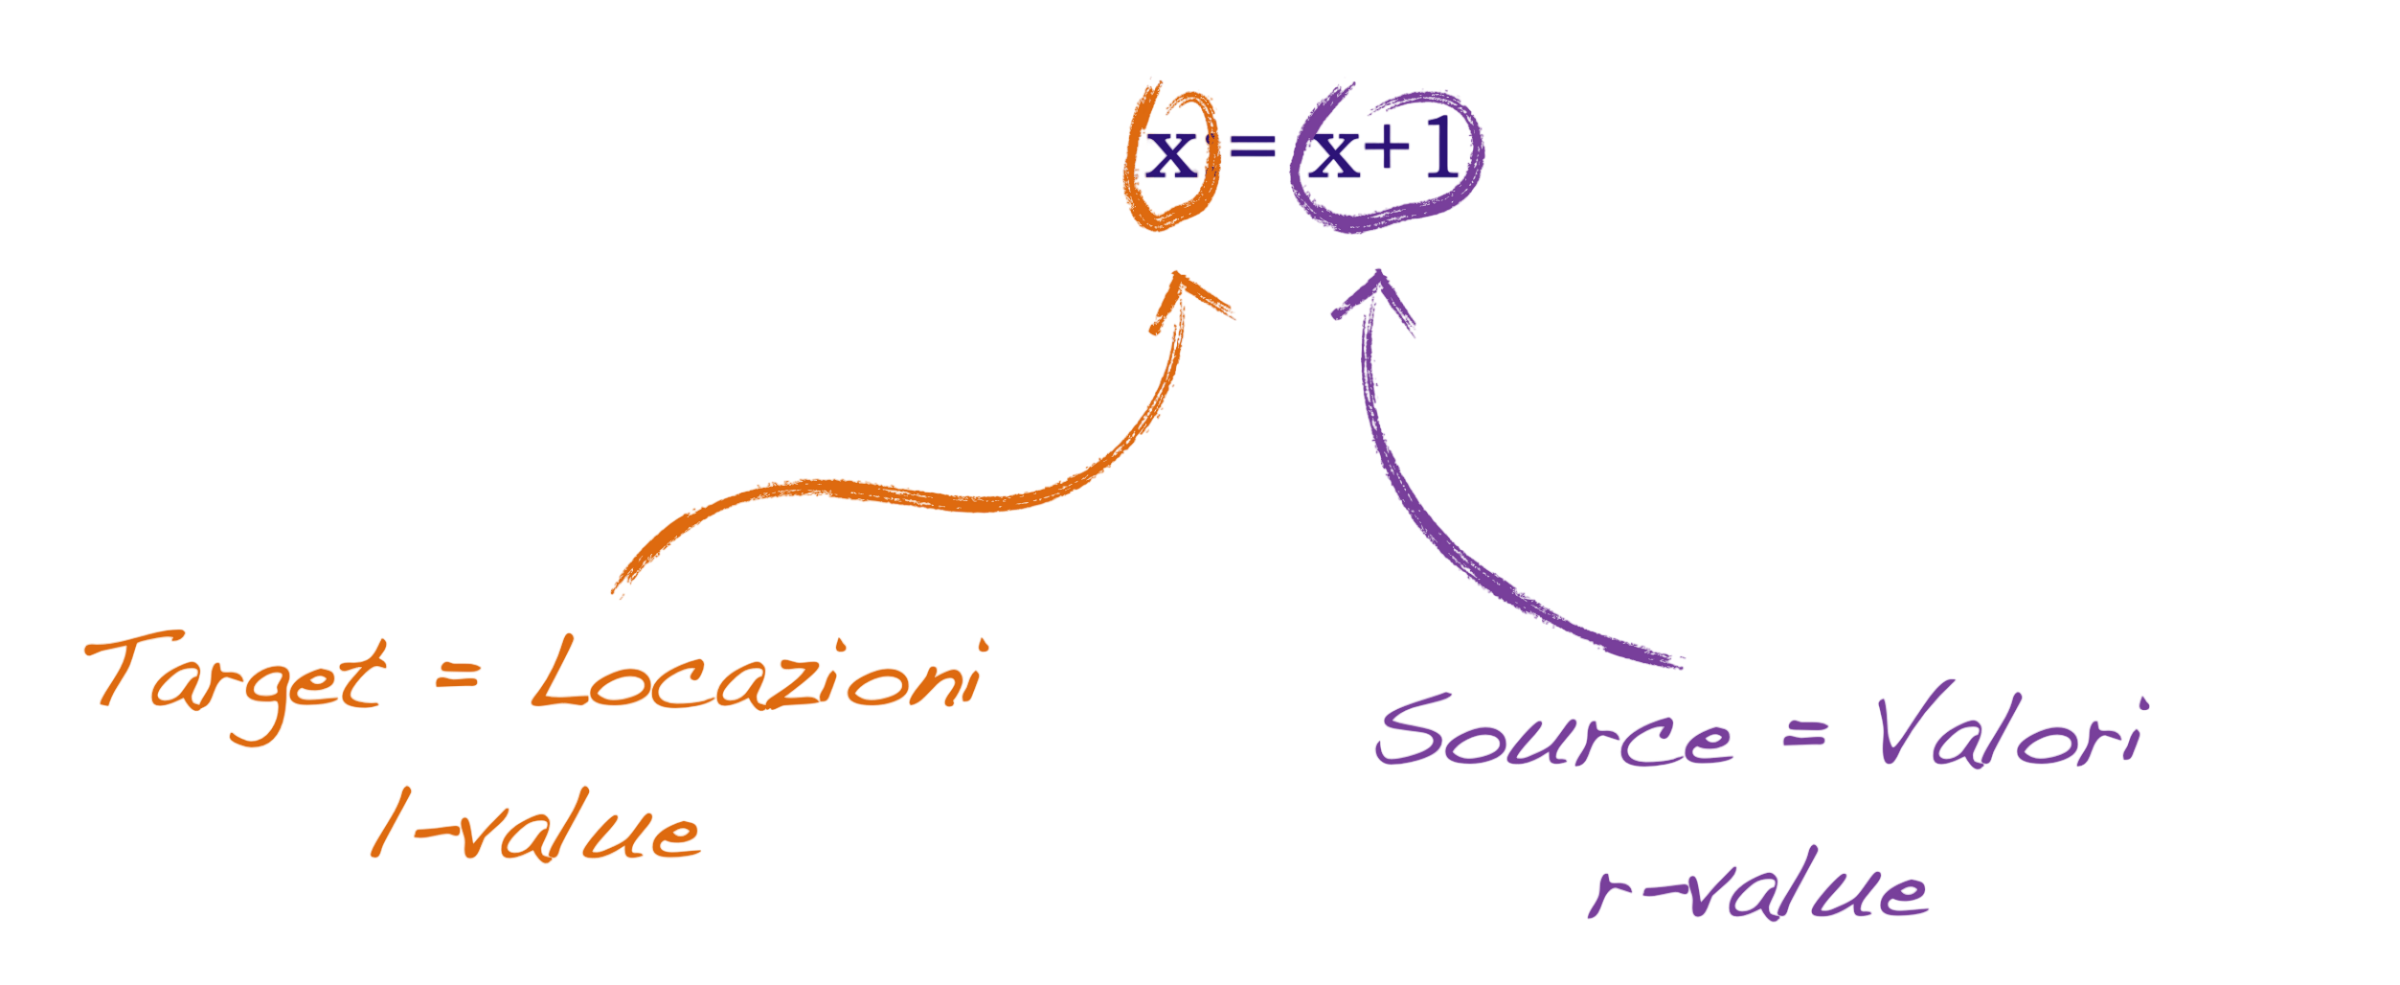
\includegraphics[width=0.55\textwidth]{images/assegnamento.png}
\end{figure}

\section{Semantica}
Definiamo gli identificatori liberi e definiti:
\[
    \begin{aligned}
        \mathrm{FI}(\texttt{x := e}) &= \mathrm{FI(\texttt{e})} \cup \{\mathrm{x}\}\\
        \mathrm{DI(\texttt{x := e})} &= \emptyset 
    \end{aligned}
\]

\subsection{Semantica statica}
La semantica statica per i comandi serve solo a verificare che il comando sia ben formato, ovvero rsipetti tutti i vincoli semantci del comando.\\[0.2ex]
Con la seguente notazione diciamo che il comando \texttt{c} è ben formato nell'ambiente statico $\Delta$, definito sull'insieme di identificatori $\mathrm{V}$:
\[
    \mathbf{\Delta \vdash_V c}
\]

L'assegamento è ben formato se l'identificatore a sinistra del simbolo di assegnamento è un identificatore variabile, e se è del tipo dell'espressione assegnata.\\[0.2ex]
Dobbiamo, quindi, valutare il tipo $\tau$ dell'espressione nello stesso ambiente statico e questo deve coincidere con il tipo associato dall'ambiente all'identificatore, che deve essere $\tau\text{loc}$.

\vario{Regola $\mathcal{C}_{\mathrm{S}_0}$}{
    \[
        \mathcal{C}_{\mathrm{S}_0}: \ \vdash \texttt{skip} \text{ (nessun vincolo da rispettare)}
    \]
}

\vario{Regola $\mathcal{C}_{\mathrm{S}_1}$}{
    \[
        \mathcal{C}_{\mathrm{S}_1}:\;
        \begin{prooftree}
            \hypo{\Delta \vdash_\mathrm{V} \mathrm{e} : \tau}
            \infer1{\Delta \vdash_\mathrm{V} \mathrm{x} := \tau}
        \end{prooftree}
        \quad \Delta(x) = \tau\text{loc}
    \]
}

\esempio{semantica statica}{

}


\subsection{Semantica dinamica}
Per la semantica dinamica dobbiamo valutare, per prima cosa, l'espressione.

\vario{Regola $\mathcal{C}_1$}{
    \[
        \mathcal{C}_1:\;
        \begin{prooftree}
            \hypo{\rho \vdash_\Delta \langle \mathrm{e}, \sigma \rangle \to_\mathrm{e} \langle \mathrm{e}', \sigma \rangle}
            \infer1{\rho \vdash_\Delta \langle \texttt{x := e}, \sigma \rangle \to_\mathrm{c} \langle \texttt{x := e'}, \sigma \rangle}
        \end{prooftree}
    \]
}

Una volta che l'espressione è completamente valutata, possiamo aggiornare la memoria associando a \texttt{x} il nuovo valore ottenuto e restituire, quindi, la memoria come configurazione terminale.

\vario{Regola $\mathcal{C}_2$}{
    \[
        \mathcal{C}_2 : \rho \vdash \langle \texttt{x := k}, \sigma \rangle    \to_\mathrm{c} \sigma[l \gets k] \quad \rho(\mathrm{x}) = 1
    \]
}

\esempio{semantica dinamica}{

}

\section{Strutture di controllo}

\subsection{Comandi di selezione}
I comandi di selezione forniscono gli strumenti per sceggliere tra due o più cammini di esecuzione:
\begin{itemize}[label=$\triangleright$, itemsep=\smallskipamount]
    \item \textbf{selettori a due vie} (\texttt{if-then-else})
    \item \textbf{selettori a più vie} (\texttt{switch-case})
\end{itemize}

\subsubsection{Selettori a due vie}
I comandi condizionali presentano la seguente sintassi:
\begin{bnfcode}{Sintassi comandi condizionali}
    if B then C else C
\end{bnfcode}

Prima, però, vediamo in che posizione si trovano gli identificatori dentro questo costrutto:
\[
    \begin{aligned}
        \mathrm{FI}(\texttt{if B then C else C}) &= \mathrm{FI}(\texttt{B}) \cup \mathrm{FI}(\texttt{C}) \cup \mathrm{FI}(\texttt{C})\\
        \mathrm{DI}(\texttt{if B then C else C}) &= \mathrm{DI}(C) \cup \mathrm{DI}(\texttt{C})
    \end{aligned}
\]

\paragraph{Semantica statica}
La semantica statica deve verificare se il comando è ben formato.\\[0.2ex]
In questo caso i vincoli da verificare saranno che l'espressione sia di tipo booleano e che i comandi dei rami condizionali siano ben formati.

\vario{Regola $\mathcal{C}_{\mathrm{S}_2}$}{
    \[
        \mathcal{C}_{\mathrm{S}_2}:\;
        \begin{prooftree}
            \hypo{\Delta \vdash_\mathrm{V} \ \texttt{e : bool} \quad \Delta \vdash_\mathrm{C} \mathrm{c}_0 \quad \Delta \vdash_\mathrm{V} \mathrm{c}_1}
            \infer1{\Delta \vdash_\mathrm{V} \texttt{if e then } \mathrm{c}_0 \texttt{ else } \mathrm{c}_1}
        \end{prooftree}
    \]
}

\esempio{semantica statica}{

}

\paragraph{Semantica dinamica}
La semantica dinamica valuta l'espressione di guardia e se questa è \texttt{true}, allora si scieglie di proseguire l'esecuzione con $\mathrm{c}_0$, altrimenti si prosegue con $\mathrm{c}_1$.

\vario{Regola $\mathcal{C}_3$}{
    \[
        \mathcal{C}_3:\;
        \begin{prooftree}
            \hypo{\rho \vdash_\Delta \langle \mathrm{B}, \sigma \rangle \to^*_\mathrm{e} \texttt{true}, \sigma \rangle}
            \infer1{\rho \vdash_\Delta \langle \texttt{if B then C else C}, \sigma \rangle \to_\mathrm{c} \langle \texttt{if true then $c_1$ else $c_2$}, \sigma\rangle}
        \end{prooftree}
    \]
}

\vario{Regola $\mathcal{C}_4$}{
    \[
        \mathcal{C}_4 : \rho \vdash_\Delta \langle \texttt{if true then $c_0$ else $c_1$}, \sigma \rangle \to_\mathrm{c} \langle c_0, \sigma \rangle
    \]
}

\vario{Regola $\mathcal{C}_5$}{
    \[
        \mathcal{C}_5 : \rho \vdash_\Delta \langle \texttt{if false then $c_0$ else $c_1$}, \sigma \rangle \to_\mathrm{c} \langle c_0, \sigma \rangle
    \]
}

\esempio{semantica dinamica}{

}


\subsubsection{Selettori a più vie}

\subsection{Composizione}
Prima di aggiungere altri comandi, abbiamo bisogno di comporre comandi in modo sequenziale.

\smallskip
La composizione sequenziale, donotata dal "\texttt{;}" permette di specificare in modo diretto la composizione di comandi deontando il fatto che il comando a destra del simbolo di composizione inizia dopo che il comando a sinistra ha completato l'esecuzione.
\[
        \mathbf{C ; C}
\]

La composizione non altera gli identificatori in posizione sia di definizione che liberi, che, quindi, saranno l'unione di quelli dei comandi:
\[
    \begin{aligned}
        \mathrm{FI}(\texttt{$\mathrm{c_0}$ ; $\mathrm{c_1})$} &= \mathrm{FI(c_0)} \cup \mathrm{FI(c_1)}\\
        \mathrm{FI(\texttt{$\mathrm{c_0}$ ; $\mathrm{c_1}$})} &= \mathrm{DI(c_0)} \cup \mathrm{DI(c_1)}
    \end{aligned}
\]

\subsubsection{Semantica statica}
Per la semantica statica si verifica che i comandi composti siano ben formati.

\vario{Regola $\mathcal{C}_{\mathrm{S}_3}$}{
    \[
        \mathcal{C}_{\mathrm{S}_3}:\;
        \begin{prooftree}
            \hypo{\Delta \vdash_\mathrm{V} \mathrm{c}_0 \quad \Delta \vdash_\mathrm{V} \mathrm{c}_1}
            \infer1{\Delta \vdash_\mathrm{V} \mathrm{c}_0 : \mathrm{c}_1}
        \end{prooftree}
    \]
}

\vario{Regola $\mathcal{C}_{\mathrm{S}_4}$}{
    \[
        \mathcal{C}_{\mathrm{S}_4} : \Delta \vdash_\mathrm{V} \texttt{skip}
    \]
}

\subsubsection{Semantica dinamica}
Per la semantica dinamica, lo \texttt{skip} lasca inalterata la memoria, mentre la compozione esegue $\mathrm{c}_0$ e poi a partire dalla memoria risultante esegue $\mathrm{c}_1$.

\vario{Regola $\mathcal{C}_6$}{
    \[
        \mathcal{C}_6 : \rho \vdash_\Delta \langle \texttt{skip}, \sigma \rangle \to_\mathrm{c} \sigma
    \]
}

\vario{Regola $\mathcal{C}_7$}{
    \[
        \mathcal{C}_7:\;
        \begin{prooftree}
            \hypo{\rho \vdash_\Delta \langle \mathrm{c}, \sigma \rangle \to_\mathrm{c} \langle \mathrm{c}', \sigma \rangle}
            \infer1{\rho \vdash_\Delta \langle \mathrm{c} ; \mathrm{c}_0, \sigma \rangle \to_\mathrm{c} \langle \mathrm{c}' ; \mathrm{c}_0, \sigma \rangle}
        \end{prooftree}
    \]
}

\vario{Regola $\mathcal{C}_8$}{
    \[
        \mathcal{C}_8:\;
        \begin{prooftree}
            \hypo{\rho \vdash_\Delta \langle \mathrm{c}, \sigma \rangle \to_\mathrm{c} \sigma'}
            \infer1{\rho \vdash_\Delta \langle \mathrm{c} ; \mathrm{c}_0, \sigma \rangle \to_\mathrm{c} \langle \mathrm{c}_0, \sigma' \rangle}
        \end{prooftree}
    \]
}

\subsection{Comandi iterativi}
L'iterazione e la ricorsione sono due meccanismi che permettono di ottenere formalismi di calcolo di Turing completi, senza di essi avremmo solo automi a stati finiti.

\smallskip
In genrale, si parla di \textbf{iterazione indeterminata} quando i cicli sono controllati logicamente, ovvero su un'espressione booleana (\texttt{while, repeat, ...}).\\[0.2ex]
Si parla, invece, di \textbf{iterazione determinata} quando i cicli sono controllati numericamente, con numero di ripetizioni del ciclo determinate al momento dell'inizio del ciclo (\texttt{for, do, ...}).

\smallskip
Vediamo per prima cosa in che posizione si trovano gli identificatori dentro questo costrutto:
\[
    \begin{aligned}
        \mathrm{FI(\texttt{while e do c})} &= \mathrm{FI(c)} \cup \mathrm{e}\\
        \mathrm{DI(\texttt{while e do c})} &= \mathrm{DI(c)}
    \end{aligned}
\]

\subsubsection{Semantica statica}
La semantia statica deve verificare se il comando è ben formato.\\[0.2ex]
In questo caso i vincoli da verificare saranno che l'espressione sia di tipo booleano e che il comando nel corpo sia ben formato.

\vario{Regola $\mathcal{C}_{\mathrm{S}_5}$}{
    \[
        \mathcal{C}_{\mathrm{S}_5}:\;
        \begin{prooftree}
            \hypo{\Delta \vdash_\mathrm{V} \ \texttt{e : bool} \quad \Delta \vdash_\mathrm{V} \mathrm{c}}
            \infer1{\Delta \vdash_\mathrm{V} \texttt{while e do c}}
        \end{prooftree} 
    \]
}

\subsubsection{Semantica dinamica}

\vario{Regola $\mathcal{C}_9$}{
    \[
        \mathcal{C}_9:\;
        \begin{prooftree}
            \hypo{\rho \vdash_\Delta \langle \mathrm{e}, \sigma \rangle \to^*_\mathrm{e} \langle \texttt{true}, \sigma \rangle}
            \infer1{\rho \vdash_\mathrm{\Delta} \langle \texttt{while e do c}, \sigma \rangle \to_\mathrm{c} \langle \texttt{c ; while e do c}, \sigma \rangle}
        \end{prooftree}
    \]
}

\vario{Regola $\mathcal{C}_{10}$}{
    \[
        \mathcal{C}_{10}:\;
        \begin{prooftree}
            \hypo{\rho \vdash_\Delta \langle \mathrm{e}, \sigma \rangle \to^*_\mathrm{e} \langle \texttt{false}, \sigma \rangle}
            \infer1{\rho \vdash_\mathrm{\Delta} \langle \texttt{while e do c}, \sigma \rangle \to_\mathrm{c} \sigma}
        \end{prooftree}
    \]   
}